\section{Introduction - The essence of learning}

Learning or development of any intelligent agent can be divided into 2 successive phases -
\begin{enumerate}
  \item Understanding or finding the target task. (Goal Discovery)
  \item Learning the task itself.
\end{enumerate}
These phases,  as shown in Figure~\ref{fig:LearningPhases},  need to be accomplished in a sequential manner.
Most of the work in contemporary machine learning has assumed that the task to accomplish is already given and understood.
All that remains is to program the computing agent to learn the task.
For example,  to find fraud in bank transactions,  it is clear that the main objective is the classification of transactions as good and bad.
The main question that remains is - How do we learn the best classifier?
Interestingly,  the learning processes of the classifier is also determined by the choice of the machine learning model e.g.  ANN,  
Random Forest Classifier etc.

\begin{figure}[htb]
  \centering
    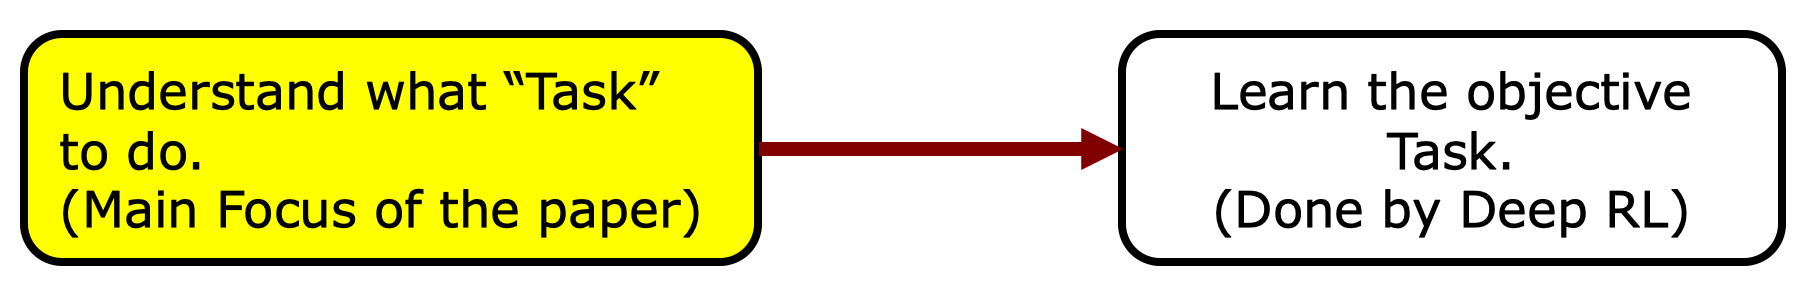
\includegraphics[width=1.0\textwidth]{img/LearningPhases}
    \caption{Learning Stages.}
    \label{fig:LearningPhases}
\end{figure}

Even though the selection of the ML models is automated to some extent using AutoML,
this methodology fails for the sequential decision making tasks. 
For solving this issue, Reinforcement Learning was developed as a general learning paradigm.
Notice, however, that RL still only  deals with the second phase of learning.
This is because the task to learn is intrinsically provided to the agent in the form of a reward function.

The authors of this paper,  in contrast, focus mainly on the first phase of learning.
They propose an agent architecture that not only learns multiple skills but also generalizes learning to new skills.
Thus their agent is an open-ended multi-skill learning agent.
They use (Deep) RL to their advantage for the second phase of learning as it is a general learning paradigm.
Hence the agent has to learn to formulate the goal as a reward function.
Subsequently it has to use the reward function to learn the task.

\section{Motivation}

The inspirations of this paper come from 2 sources, namely,  \textit{Developmental Machine Learning} and \textit{Theory of Zone of proximal development}.
% The principles taken from these 2 sources act as pillars upon which the agent's learning mechanism is built.

\subsection{Developmental Machine Learning}
This is a part of machine learning that tries to mimic the ways infants try to learn new skills.
According to psychologists,  the way infants get their internal satisfaction or reward is by accomplishing novel goals.
For example in Figure~\ref{fig:kindPlayingBlock}, after learning how to build a block-tower the child is no longer interested in repeating this task.
Even accomplishing a similar task like building a tower of books is also not very interesting or satisfying.
Novelty of the task is essential !


\begin{figure}[!tbp]
  \centering
  \begin{minipage}[b]{0.3\textwidth}
    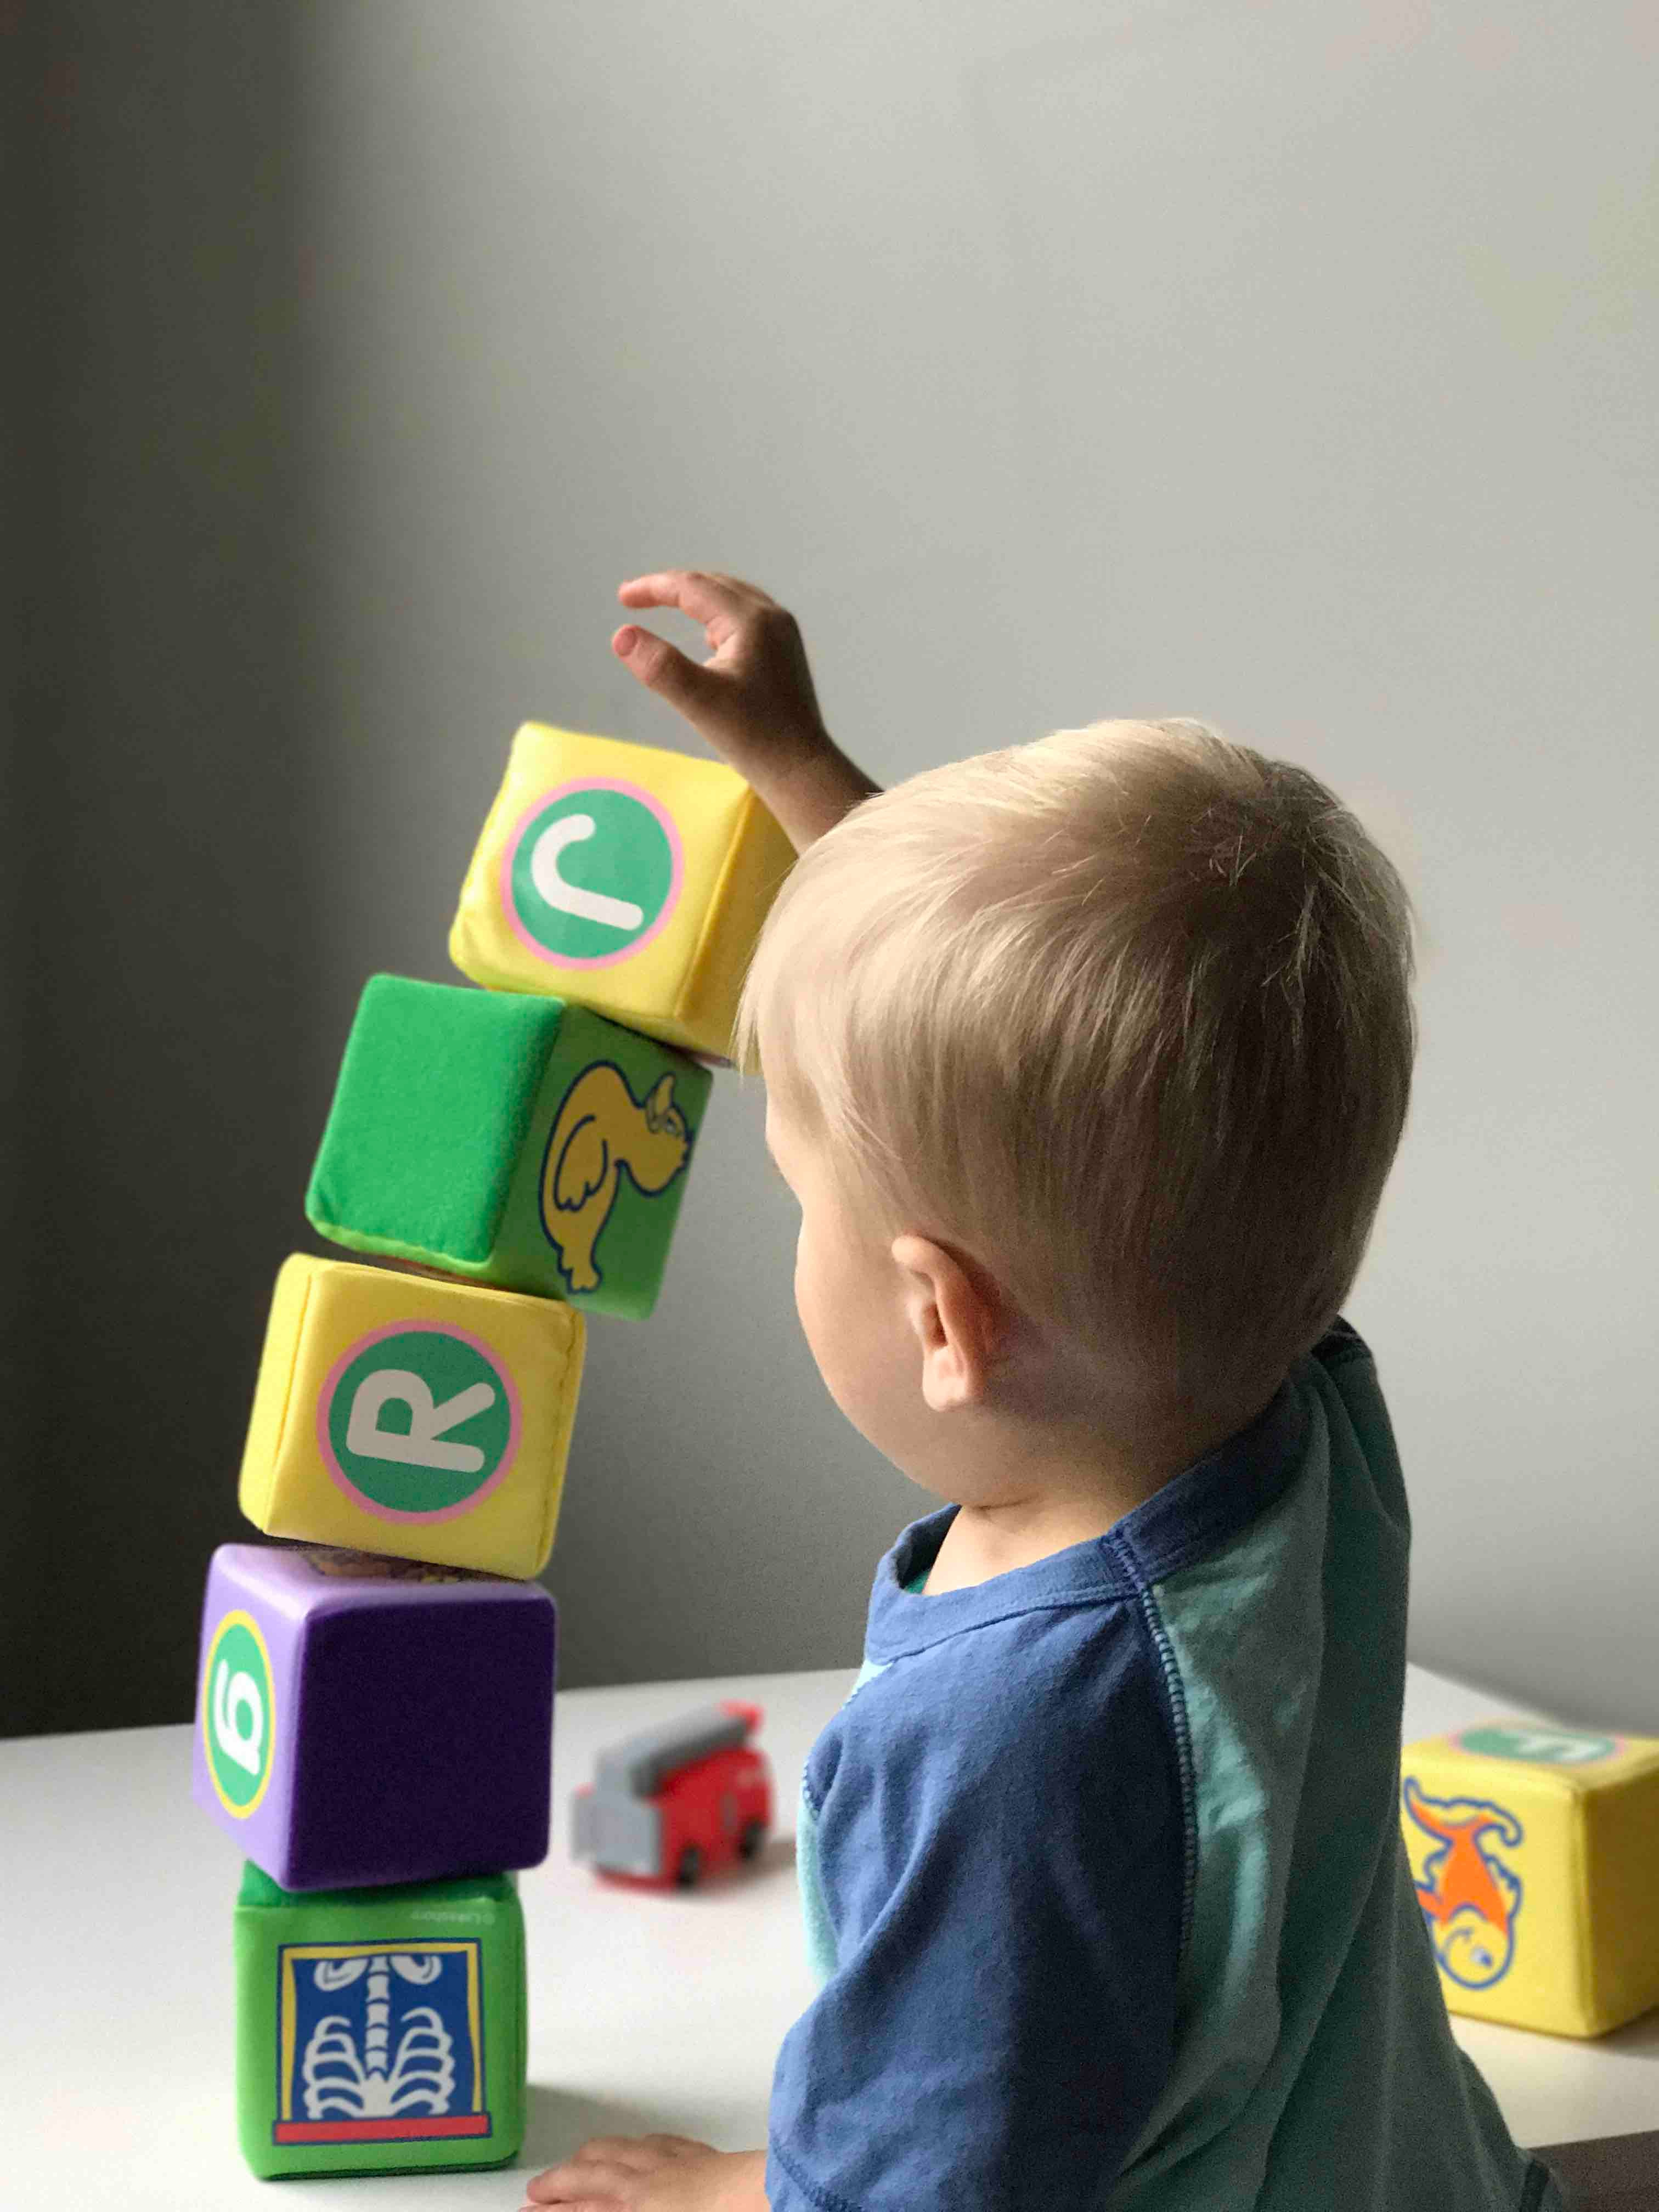
\includegraphics[width=1.0\textwidth]{img/kindPlayingBlock}
    \caption{A kid playing with blocks~\cite[p.~3]{kindPlayingBlock}.}
    \label{fig:kindPlayingBlock}
  \end{minipage}
  \hfill
  \begin{minipage}[b]{0.45\textwidth}
    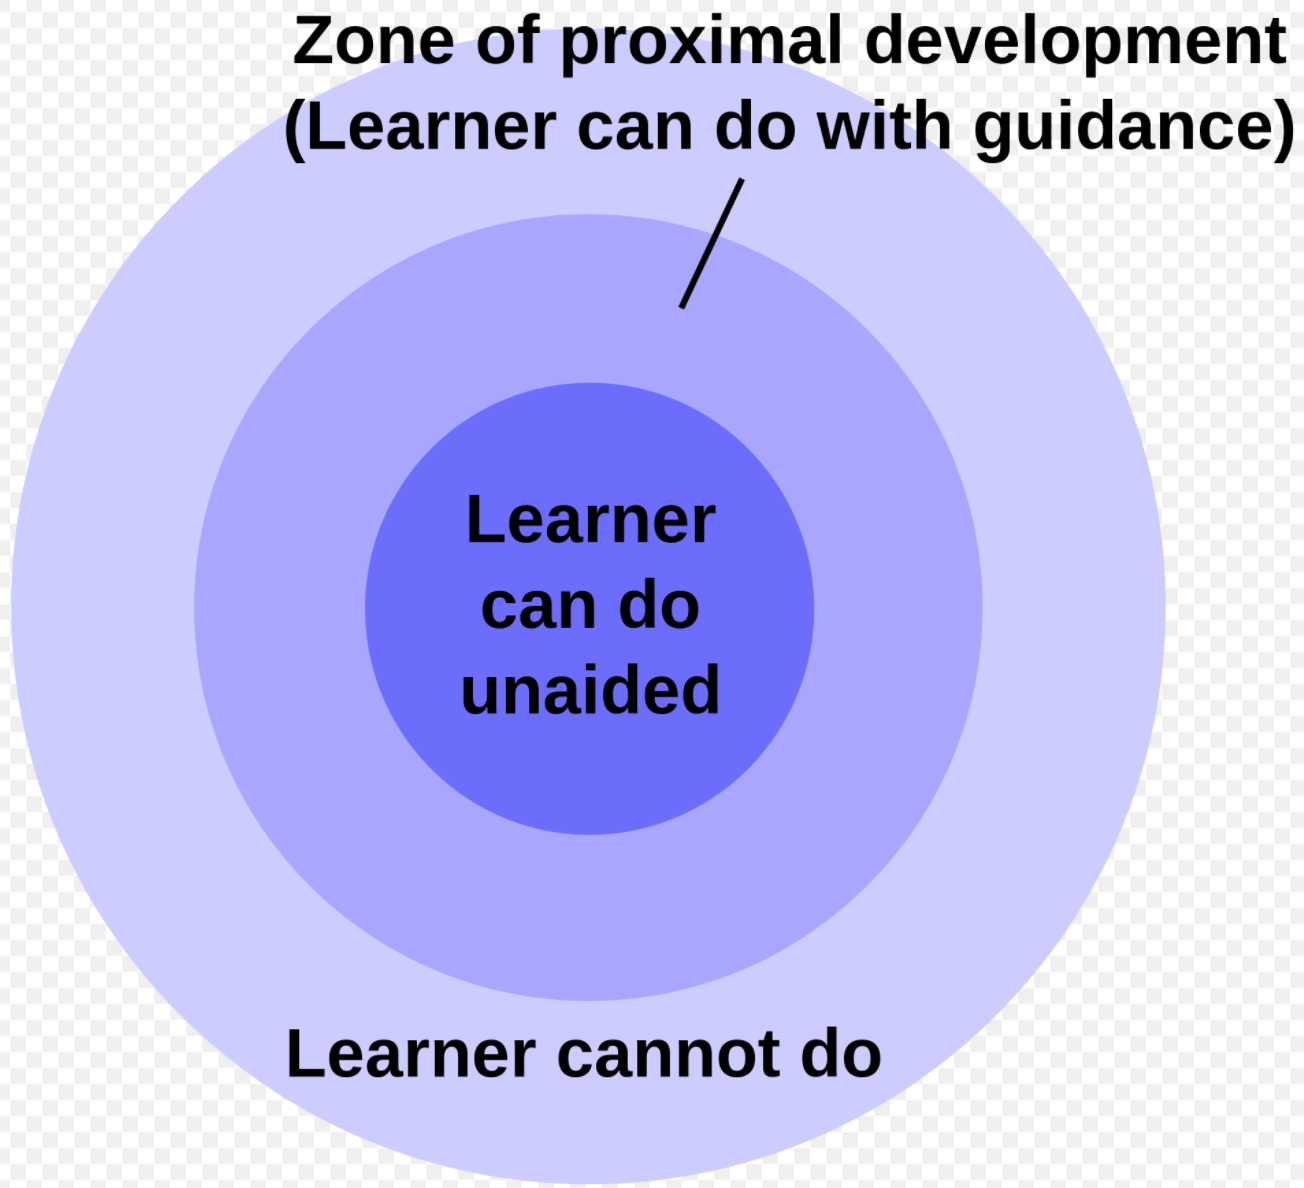
\includegraphics[width=1.0\textwidth]{img/ZPD}
    \caption{ZDP~\cite[p.~3]{ZPD}.}
    \label{fig:ZPD}
  \end{minipage}
\end{figure}

Hence psychologists say that children are intrinsically motivated or curious.
The authors try to mimic this in the "Curiosity Driven Exploration" of their agent.
They use construction grammar [See \ref{ConstructionGrammarSection}] as a mechanism to explore new goals.

\subsection{Theory of Zone of Proximal Development}
This theory,  developed by Russian psychologist Vygotsky,  says that there exist 3 zones of skills for any learner at any stage of development.
Figure~\ref{fig:ZPD} shows an illustration of these zones.
The internal zone consists of skills that the learner can learn on his own.
E.g. The child will be able to generalize building a stack of books after he learns how to build a stack of blocks.
The middle zone,  aka \textit{Zone of Proximal Development},  consists of skills that the learner can accomplish only with the help of some guidance.
E.g.  The child can learn how to build a pyramid, but he would require some guidance for this.
The outermost zone consists of skills that cannot be accomplished even with the help of guidance.
E.g.  Building a ship structure using lego blocks is beyond the child's capability regardless of the guidance given.

The key idea is this - there has to be someone to guide the child.
This is identical to the parent-child learning dynamics.
Using this principle, the authors propose the use of a social partner to guide the learning of their proposed agent.

\section{Goal Generation and Generalization}
\subsection{Previous works and their limitations}
In the previous works and in this work,  each goal is given by $g \in \mathbf{R}^m$.
Using a set of known Goals $G$,  previous papers trained models such as \textit{Adversarial Neural Networks} and \textit{Variational Auto-Encoders}.
Using these models,  new goals within the known/seen distribution were created.
This is a limitation because it is not a novel goal for the agent.
E.g. The tasks - Building a stack of blocks and a stack of books are within the same goal distribution.
But they are not novel for the child.
What is novel is to jump to building a pyramid which is an out of distribution Goal.
The authors try to overcome this limitation by using language for generating new goals instead of the above generative models.

\subsection{Goal Generation Mechanism - Construction Grammar}
\label{ConstructionGrammarSection}

The authors make use of a concept called Construction Grammar to generate new goals.
Using Construction Grammar it is able to generate out of known distribution goals.
Each word, being \textbf{semantically undividable}, is called an atom.
Atoms combine to form compounds which are ultimately sentences describing goals.
Figure~\ref{fig:CGFundamentals} provides an example.

\begin{figure}[htb]
  \centering
    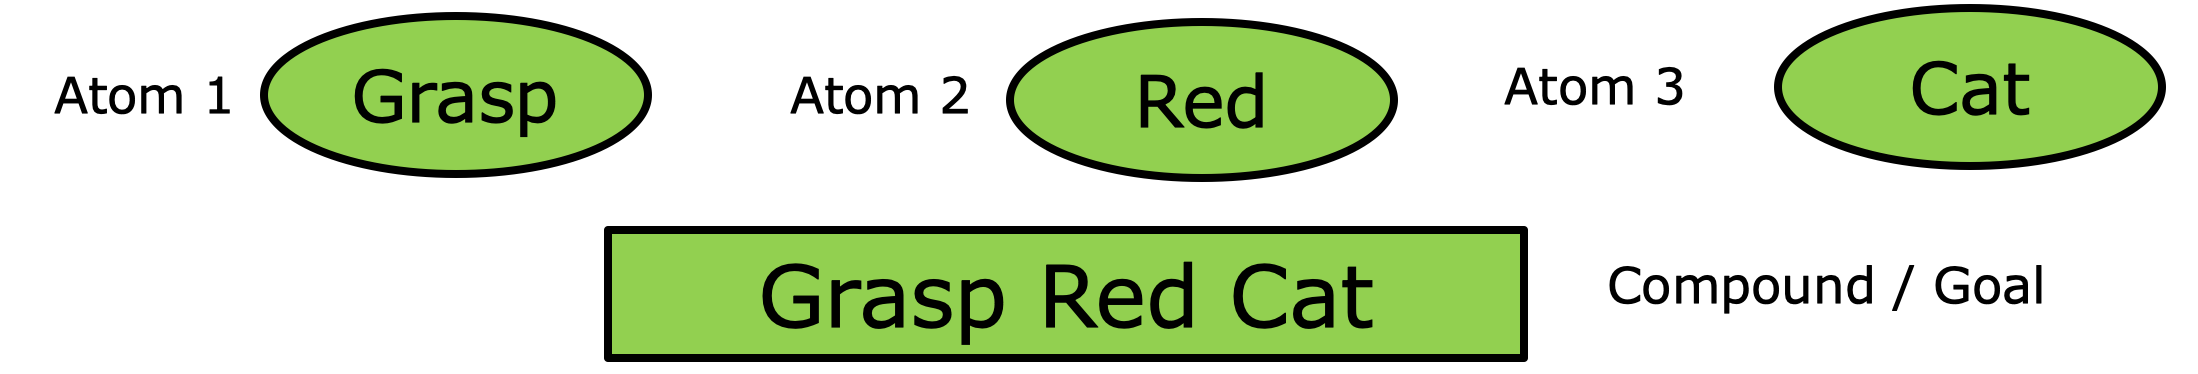
\includegraphics[width=0.8\textwidth]{img/CGFundamentals}
    \caption{Fundamental Components of Construction Grammar.}
    \label{fig:CGFundamentals}
\end{figure}

To study the effects of Goal generalization in isolation, the authors do not use a  full blow NLP agent.
They use a simple and controlled Grammar as shown in Figure~\ref{fig:ConstructionGrammarImage} .
It has 3 main actions/verbs \textbf{Go} (to a zone) \textbf{Grasp} (an object) and \textbf{Grow} (an object).
The number of objects depend on the environment complexity. [See \ref{EnvironmentSection} ]

\begin{figure}[htb]
  \centering
    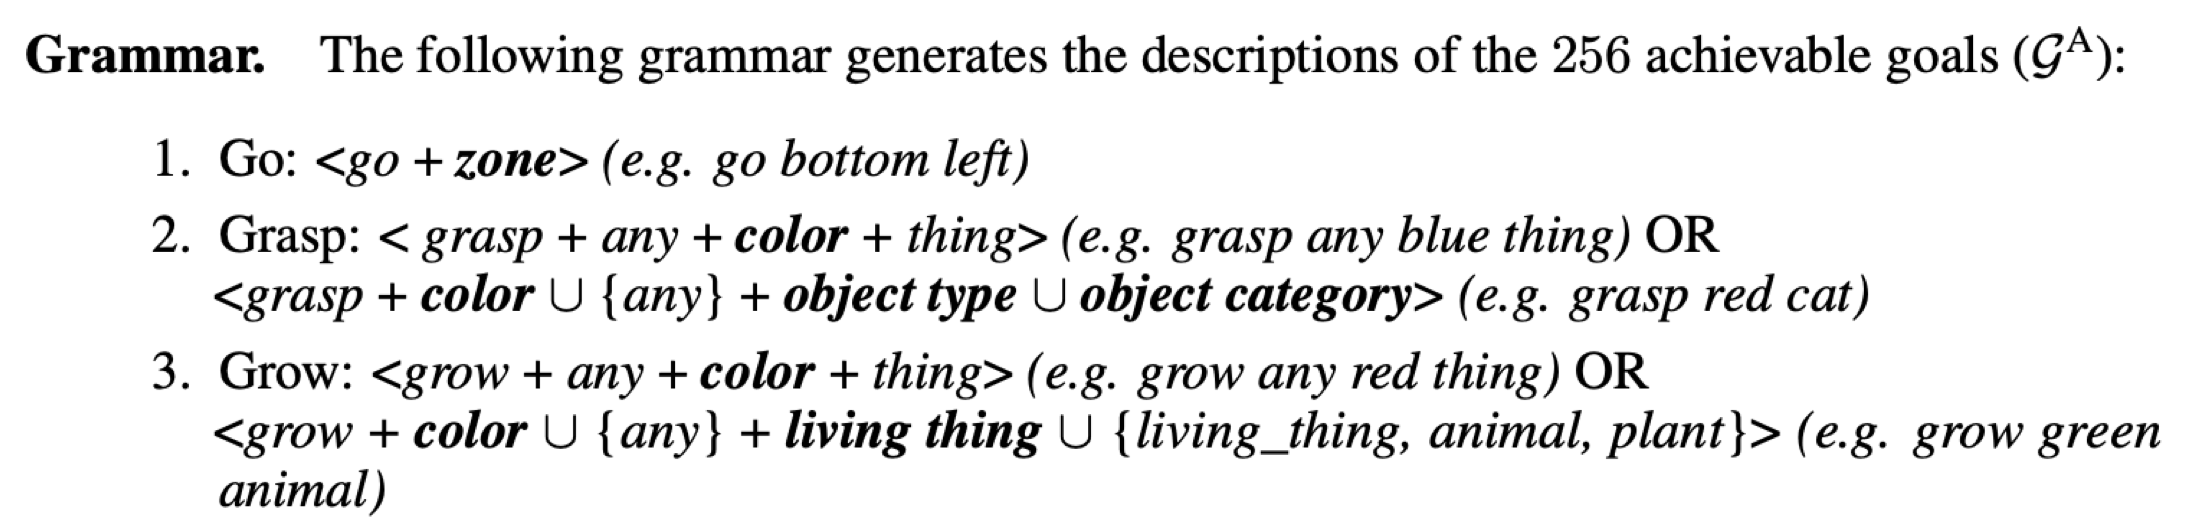
\includegraphics[width=0.8\textwidth]{img/ConstructionGrammarImage}
    \caption{Construction Grammar used in the Paper.}
    \label{fig:ConstructionGrammarImage}
\end{figure}

\subsection{Goal Generation "Curiosity" algorithm}
The essence of this algorithm is that the authors try to compute equivalent atoms.
Given 2 known goals like "Move Red Table" and "Move Red Chair", the edit distance between the goals is 1.
This is because by replacing 1 word "Table" with "Chair" we can move from the first to the second goal (and vice-versa).
Now the atoms "Table" and "Chair" are considered equivalent.
One can be replaced for another in a goal to obtain a different goal.
For example "Break Red Chair" can be converted to "Break Read Table".
The new compounds/goals formed by replacing equivalent atoms are called imagined goals.
Figure~\ref{fig:CuriosityAlgorithm} shows the complete algorithm with its essence.
Using these imagined goals, the agent explores the goal space to get better goal generalization.

\begin{figure}[htb]
  \centering
    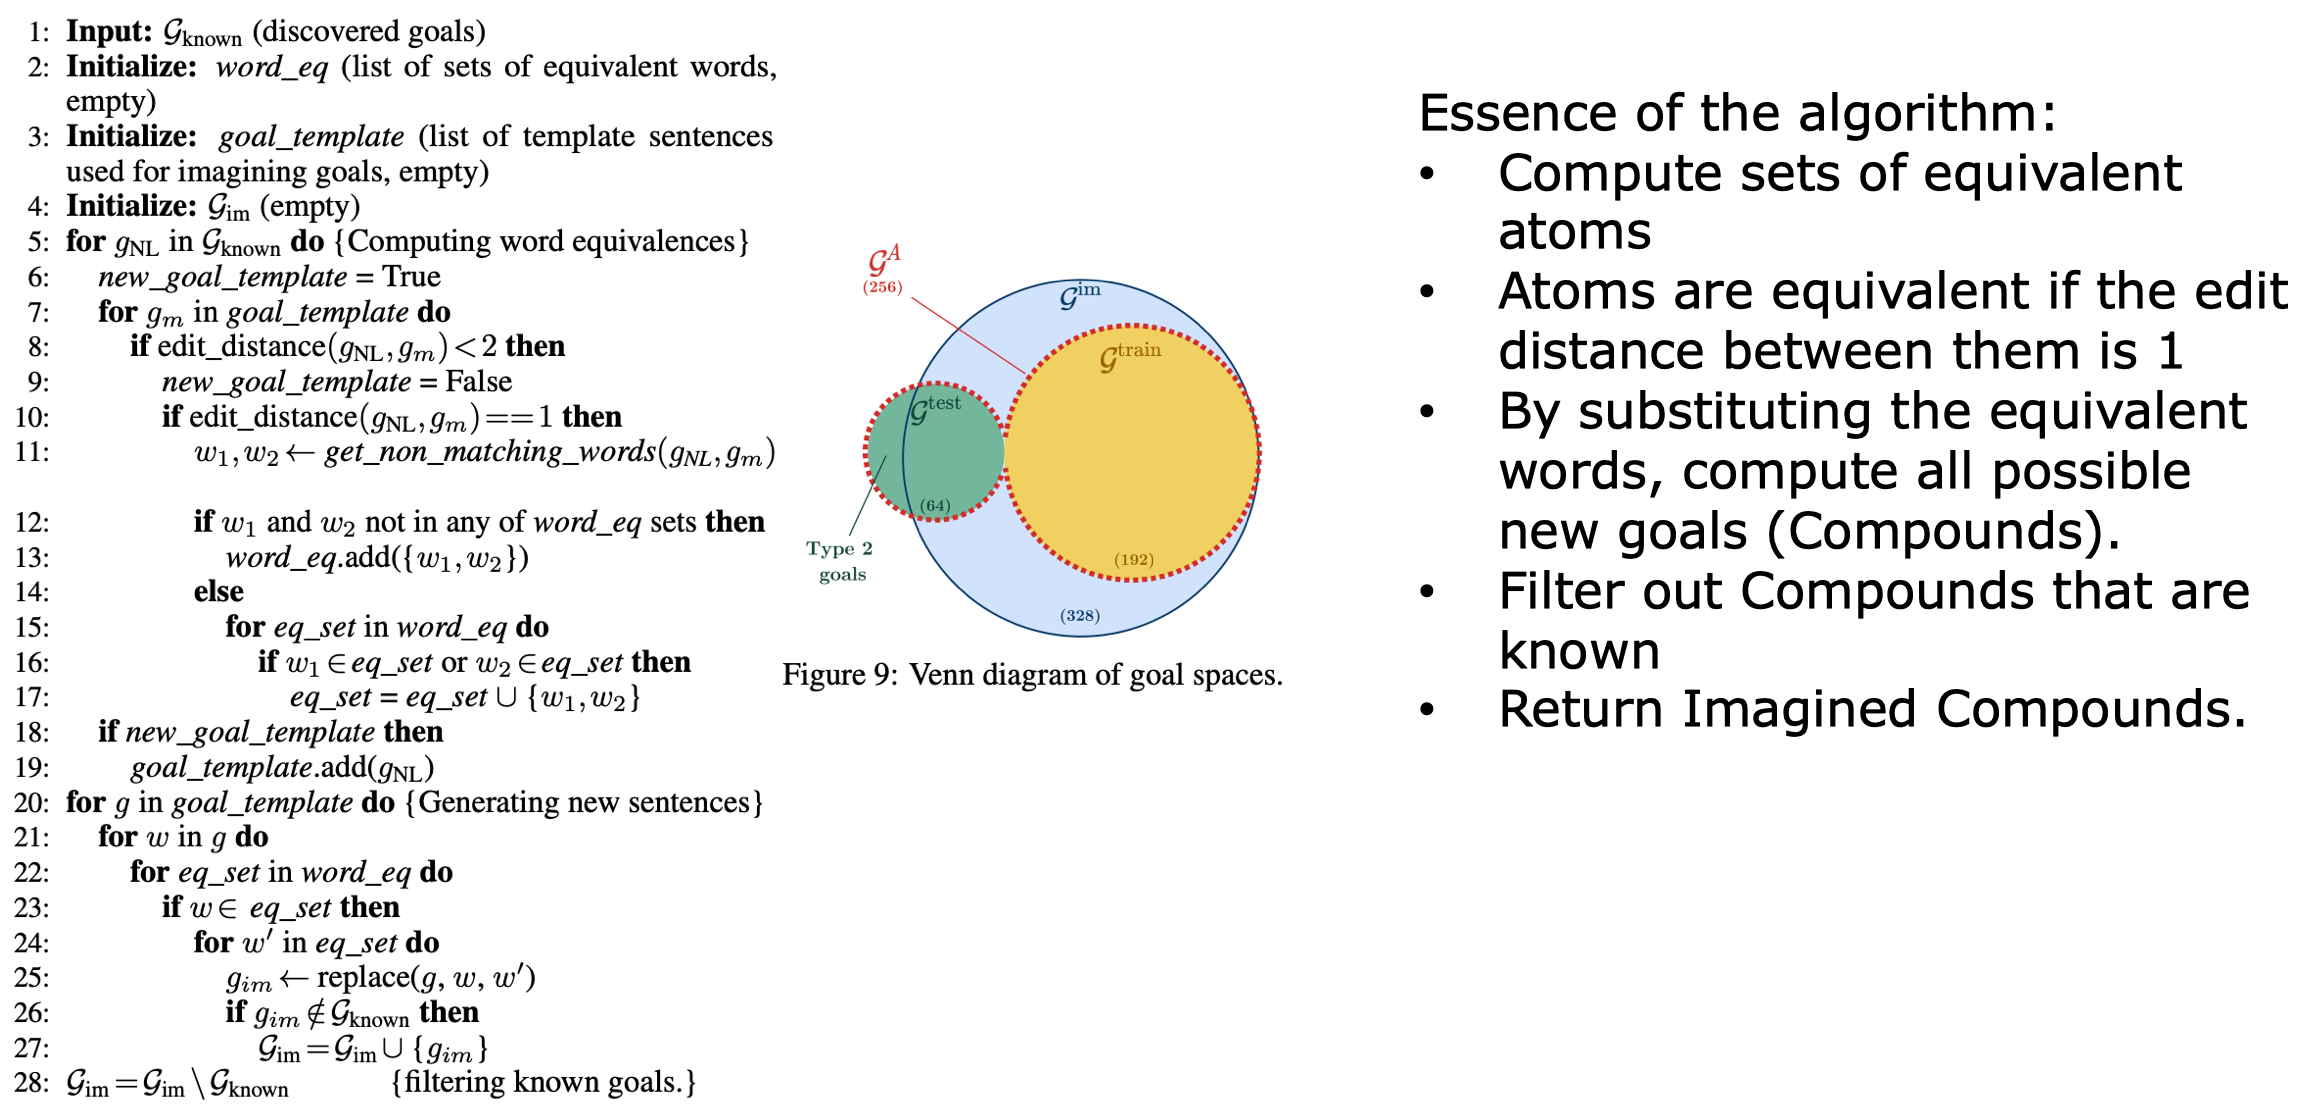
\includegraphics[width=1.0\textwidth]{img/CuriosityAlgorithm}
    \caption{Curiosity Algorithm.}
    \label{fig:CuriosityAlgorithm}
\end{figure}

\subsection{Goal Generalization vs State Space Generalization}
As there are 2 distinct phases of learning, as seen above,  so are there 2 distinct generalizations
\begin{itemize}
\item Goal Generalization - Corresponding to the Goal Discovery Phase.
\item State Space Generalization - Corresponding to the Task Learning Phase.
\end{itemize}

\begin{figure}[!tbp]
  \centering
  \begin{minipage}[b]{0.45\textwidth}
    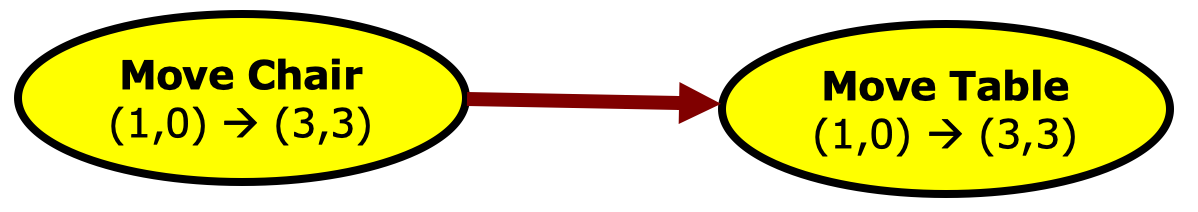
\includegraphics[width=1.0\textwidth]{img/GoalGeneralization}
    \caption{Goal Generalization}
    \label{fig:GoalGeneralization}
  \end{minipage}
  \hfill
  \begin{minipage}[b]{0.45\textwidth}
    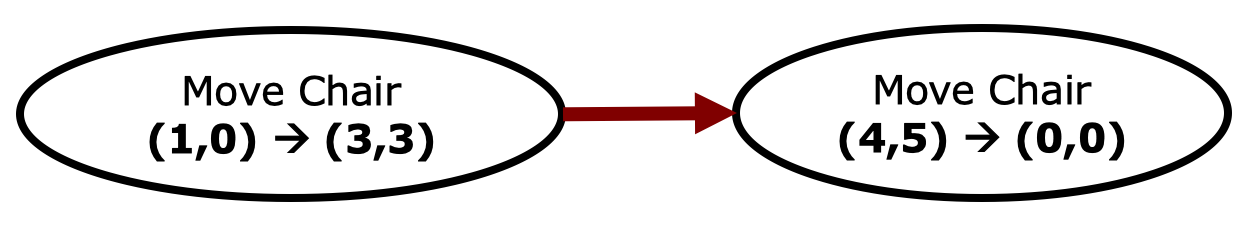
\includegraphics[width=1.0\textwidth]{img/StateSpaceGeneralization}
    \caption{State Space Generalization}
    \label{fig:StateSpaceGeneralization}
  \end{minipage}
\end{figure}

Consider a space of "Moving objects on an $x y$ plane".
Figure~\ref{fig:StateSpaceGeneralization} shows that if an agent has learnt to move 1 type of object (here a chair),  then a good State space generalization would 
be that the agent can apply this skill to move the chair between any 2 points in the $x y$ plane.
However only when an agent can move a distinct object, here a table, between the same points can we claim that the agent can 
generalize across goals. This is illustrated in Figure~\ref{fig:GoalGeneralization}.
The authors are primarily concerned with Goal Generalization in the paper.


\section{Synthetic Environment - Playground}
\label{EnvironmentSection}
Because of the complexity reasons mentioned in \ref{ConstructionGrammarSection}
the authors do not learn a full blown Perception agent.
The environment is a 2D space in which the agent and the objects are represented as circles (internally).
3 types of objects are hard coded in the environment - living things e.g. a plant,  a cat,  a lion etc., non living things e.g. a chair, a table etc. 
and supplies i.e food and water.

The objects together with the construction grammar form a virtual farm in which the agent can Grasp and move the objects and also grow the living things.
The objects can be referenced using their predicates. 
These predicates are organised in a hierarchy similar to the class hierarchy in an Object Oriented Programming language.
The predicates aid the curiosity algorithm to make bigger jumps within the goal space.
For example, "Grow red Animal" generalised to "Grow red Plant" is a huge jump in the goal space than jumping from "Grow red Cat" to "Grow red Dog".
This is because plants can only be grown with water unlike the animals that can grow with both water and food.
Figure~\ref{fig:EnvironmentLayout} shows the environment layout created in one instance.
Figure~\ref{fig:ObjectsAndHeirarchy} shows the hard coded objects in the environment used for testing.

\begin{figure}[!tbp]
  \centering
  \begin{minipage}[b]{0.35\textwidth}
    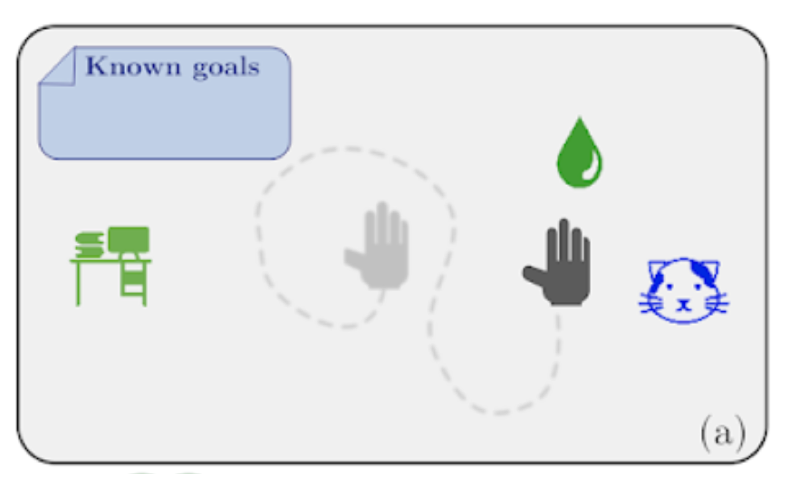
\includegraphics[width=1.0\textwidth]{img/EnvironmentLayout}
    \caption{The Playground Environment}
    \label{fig:EnvironmentLayout}
  \end{minipage}
  \hfill
  \begin{minipage}[b]{0.55\textwidth}
    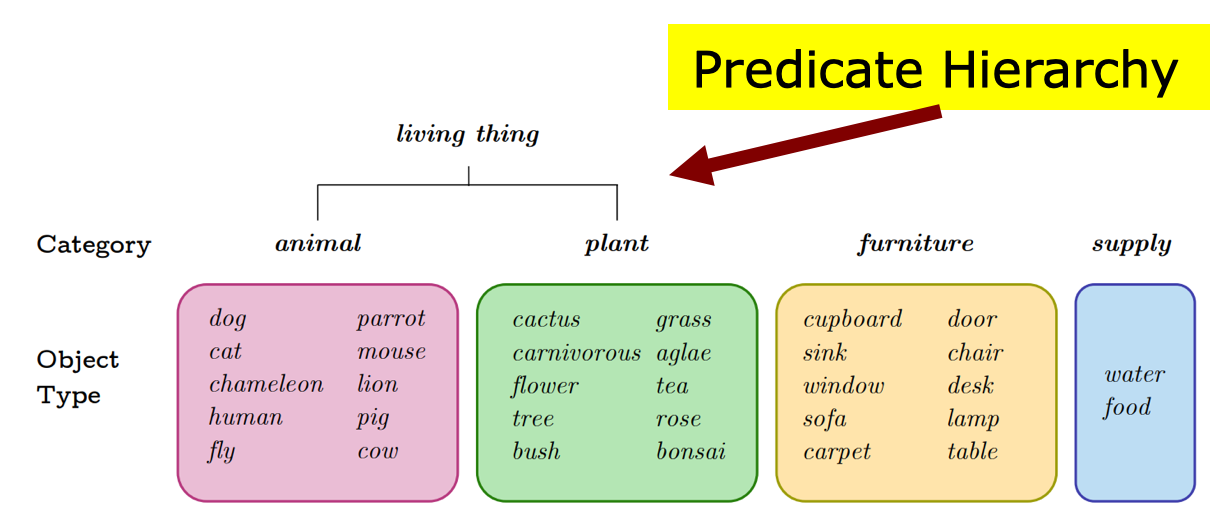
\includegraphics[width=1.0\textwidth]{img/ObjectsAndHeirarchy}
    \caption{Objects in the Environment}
    \label{fig:ObjectsAndHeirarchy}
  \end{minipage}
\end{figure}

\subsection{Environment Representations}
\label{EnvironmentRepresentationSection}
As the agent, in principle, is a Reinforcement Learning agent,  the following representations are defined for the environment - 
\begin{itemize}
\item object = $[d, r, g, b, ...] \in \mathbf{R}^n$ where $n \in \mathbf{I}^+$
\item agent = $[x, y, g]$ and action = $[\delta x, \delta y, \delta g]$
\item observation = $[$agent$]$ +$[$object$]_1$ +$[$object$]_2$ ...
\item state = $[$observation$]$ + $[\delta$observation$]$
\end{itemize}
Where $d \in \mathbf{R}$ is for diameter, $[x, y] \in \mathbf{R}^2$ is the position in 2D space,
$g \in \{-1, 1\}$ is wether an object is grasped or not by the agent and
$[r, g, b] \in \mathbf{R}^3$ represents Color.

\section{Language Encoder and function approximators}
The main functions of our RL agent i.e the Reward,  the Policy and the Critic are function approximators represented by Deep Neural Networks.
Because our agent is a multi-skilled agent, these function approximators should be conditioned on the target goal.
Because the target goal in its NL state cannot be used as a conditioner, the authors use a Long Short-Term Memory (LSTM) network to encode the goal into $\mathbf{R}^{100}$.
The LSTM network is the language encoder and is represented by the function
$L_e : g \mapsto \mathbf{R}^{100} \; \forall g \in G$ where $G$ is the set of goals obtainable from the Construction Grammar.

\subsection{Reward (R),  policy($\pi$) and Critic (Q) function approximators}
Deep Neural Network is used as a function approximator for R, $\pi$ and Q functions.
In the environment's , the features of objects can be appended to the state in any order [see \ref{EnvironmentRepresentationSection}].
Hence all the function approximators have to be permutation invariant.
This is accomplished by dividing the state into object specific parts and using permutation invariant mathematical operators like $\sum$ and \textbf{OR}.
% The reward function is learnt as a binary classifier and is defined as $R(s, g) : \mathbf{S} \times \mathbf{R}^{100} \mapsto \{0,1\} $ 


\section{Proposed Architecture}
The curiosity algorithm is an intrinsic part of the proposed architecture by the authors.
Hence the agent is intrinsically motivated.
Similarly the Social Partner is also an intrinsic part of the architecture hence there is always guidance given to the agent 
so that the agent can learn skills in its Proximal Zone of Development.

The basic idea - Run the algorithm.
Store anything that is interesting and use the data stored in the memory to 

\section{Working of the Imagine Algorithm}

\section{Goal generalization}

\section{Experiments and Results}

\subsection{Study on Goal Imagination}

\subsection{Studying the effect of changes in Social Partner}

\section{Limitations and Future Work}

\section{Critical Review}

\section{Conclusion}

\section{Garbage}

\ifx false
% Disabling this because there is no space to put this into the summary
\section{Language - A medium for Curiosity and Guidance}
The authors use Language for both goal discovery (curiosity) as well as for guidance of the agent because
\begin{itemize}
\item In the parent-child dynamics, the parent being the social partner gives guidance to the child using language.
The authors try to mimic this.
\item Languages embody collective knowledge that has developed over 1000s of years .
They contain words that explain complex concepts using sufficiently high levels of abstractions.
\item Combinatorial composition of language makes it good for formulating and imagining new goals.
This combinatorial composition aids in the development of novel goals.
\end{itemize}
\fi

\ifx false
Figure~\ref{fig:octomap}.

\begin{figure}[htb]
  \centering
    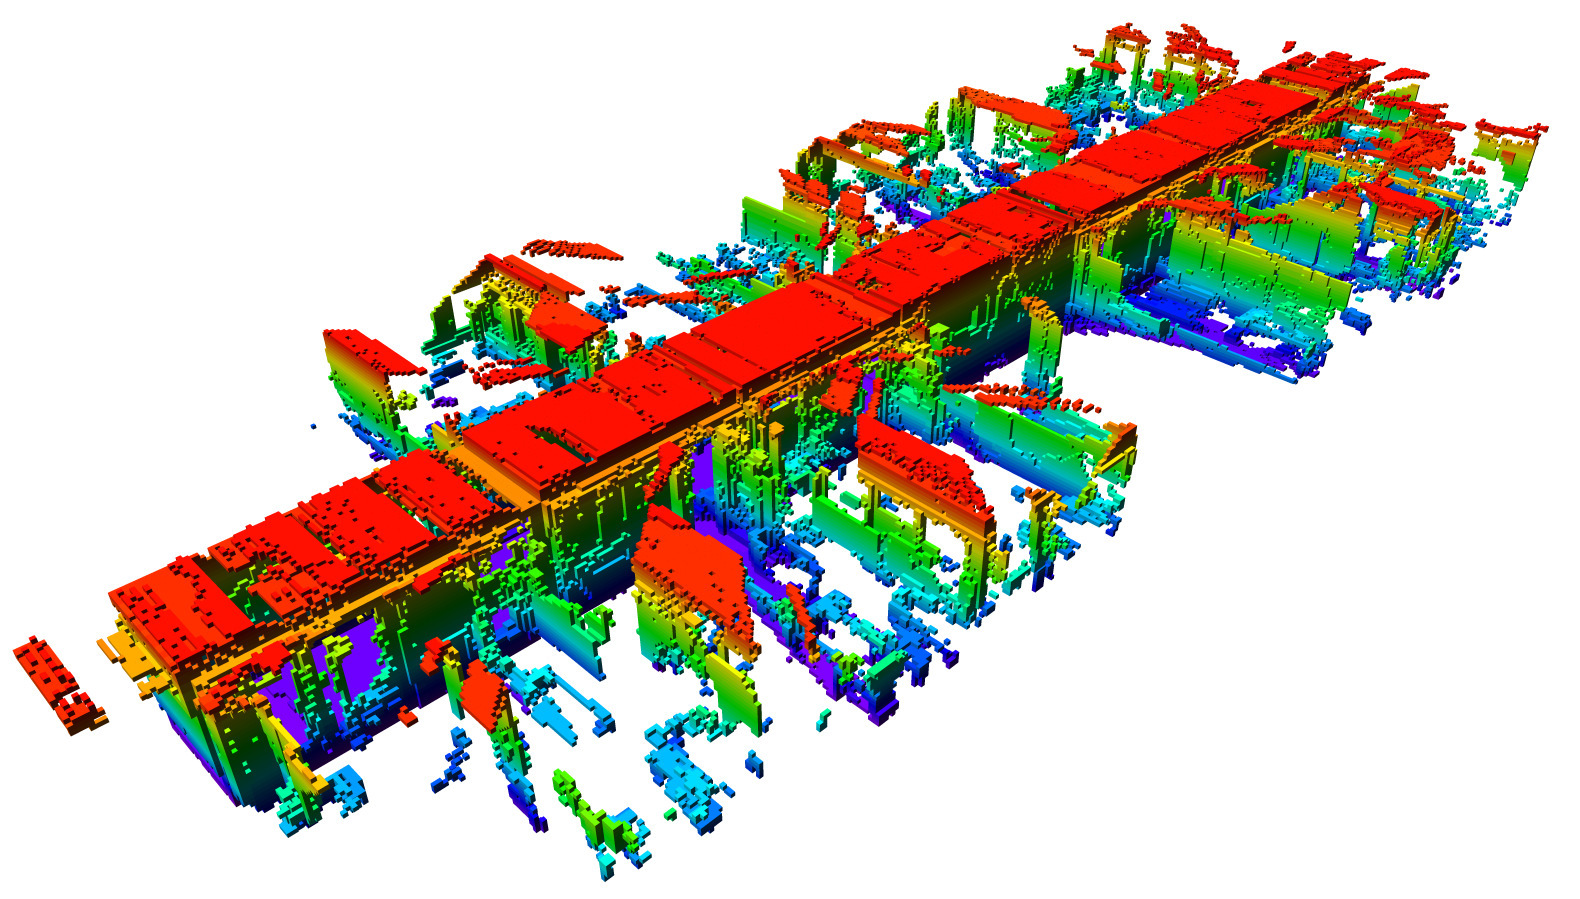
\includegraphics[width=0.5\textwidth]{img/octomap}
    \caption{A map created with the Octomap algorithm~\cite[p.~3]{wurm2010octomap}.}
    \label{fig:octomap}
\end{figure}

\begin{equation}
	\int_0^\infty e^{-x}\mathrm{d}x = 1
\end{equation}
\fi